% Options for packages loaded elsewhere
\PassOptionsToPackage{unicode}{hyperref}
\PassOptionsToPackage{hyphens}{url}
%
\documentclass[
]{article}
\usepackage{amsmath,amssymb}
\usepackage{iftex}
\ifPDFTeX
  \usepackage[T1]{fontenc}
  \usepackage[utf8]{inputenc}
  \usepackage{textcomp} % provide euro and other symbols
\else % if luatex or xetex
  \usepackage{unicode-math} % this also loads fontspec
  \defaultfontfeatures{Scale=MatchLowercase}
  \defaultfontfeatures[\rmfamily]{Ligatures=TeX,Scale=1}
\fi
\usepackage{lmodern}
\ifPDFTeX\else
  % xetex/luatex font selection
\fi
% Use upquote if available, for straight quotes in verbatim environments
\IfFileExists{upquote.sty}{\usepackage{upquote}}{}
\IfFileExists{microtype.sty}{% use microtype if available
  \usepackage[]{microtype}
  \UseMicrotypeSet[protrusion]{basicmath} % disable protrusion for tt fonts
}{}
\makeatletter
\@ifundefined{KOMAClassName}{% if non-KOMA class
  \IfFileExists{parskip.sty}{%
    \usepackage{parskip}
  }{% else
    \setlength{\parindent}{0pt}
    \setlength{\parskip}{6pt plus 2pt minus 1pt}}
}{% if KOMA class
  \KOMAoptions{parskip=half}}
\makeatother
\usepackage{xcolor}
\usepackage[margin=1in]{geometry}
\usepackage{color}
\usepackage{fancyvrb}
\newcommand{\VerbBar}{|}
\newcommand{\VERB}{\Verb[commandchars=\\\{\}]}
\DefineVerbatimEnvironment{Highlighting}{Verbatim}{commandchars=\\\{\}}
% Add ',fontsize=\small' for more characters per line
\usepackage{framed}
\definecolor{shadecolor}{RGB}{248,248,248}
\newenvironment{Shaded}{\begin{snugshade}}{\end{snugshade}}
\newcommand{\AlertTok}[1]{\textcolor[rgb]{0.94,0.16,0.16}{#1}}
\newcommand{\AnnotationTok}[1]{\textcolor[rgb]{0.56,0.35,0.01}{\textbf{\textit{#1}}}}
\newcommand{\AttributeTok}[1]{\textcolor[rgb]{0.13,0.29,0.53}{#1}}
\newcommand{\BaseNTok}[1]{\textcolor[rgb]{0.00,0.00,0.81}{#1}}
\newcommand{\BuiltInTok}[1]{#1}
\newcommand{\CharTok}[1]{\textcolor[rgb]{0.31,0.60,0.02}{#1}}
\newcommand{\CommentTok}[1]{\textcolor[rgb]{0.56,0.35,0.01}{\textit{#1}}}
\newcommand{\CommentVarTok}[1]{\textcolor[rgb]{0.56,0.35,0.01}{\textbf{\textit{#1}}}}
\newcommand{\ConstantTok}[1]{\textcolor[rgb]{0.56,0.35,0.01}{#1}}
\newcommand{\ControlFlowTok}[1]{\textcolor[rgb]{0.13,0.29,0.53}{\textbf{#1}}}
\newcommand{\DataTypeTok}[1]{\textcolor[rgb]{0.13,0.29,0.53}{#1}}
\newcommand{\DecValTok}[1]{\textcolor[rgb]{0.00,0.00,0.81}{#1}}
\newcommand{\DocumentationTok}[1]{\textcolor[rgb]{0.56,0.35,0.01}{\textbf{\textit{#1}}}}
\newcommand{\ErrorTok}[1]{\textcolor[rgb]{0.64,0.00,0.00}{\textbf{#1}}}
\newcommand{\ExtensionTok}[1]{#1}
\newcommand{\FloatTok}[1]{\textcolor[rgb]{0.00,0.00,0.81}{#1}}
\newcommand{\FunctionTok}[1]{\textcolor[rgb]{0.13,0.29,0.53}{\textbf{#1}}}
\newcommand{\ImportTok}[1]{#1}
\newcommand{\InformationTok}[1]{\textcolor[rgb]{0.56,0.35,0.01}{\textbf{\textit{#1}}}}
\newcommand{\KeywordTok}[1]{\textcolor[rgb]{0.13,0.29,0.53}{\textbf{#1}}}
\newcommand{\NormalTok}[1]{#1}
\newcommand{\OperatorTok}[1]{\textcolor[rgb]{0.81,0.36,0.00}{\textbf{#1}}}
\newcommand{\OtherTok}[1]{\textcolor[rgb]{0.56,0.35,0.01}{#1}}
\newcommand{\PreprocessorTok}[1]{\textcolor[rgb]{0.56,0.35,0.01}{\textit{#1}}}
\newcommand{\RegionMarkerTok}[1]{#1}
\newcommand{\SpecialCharTok}[1]{\textcolor[rgb]{0.81,0.36,0.00}{\textbf{#1}}}
\newcommand{\SpecialStringTok}[1]{\textcolor[rgb]{0.31,0.60,0.02}{#1}}
\newcommand{\StringTok}[1]{\textcolor[rgb]{0.31,0.60,0.02}{#1}}
\newcommand{\VariableTok}[1]{\textcolor[rgb]{0.00,0.00,0.00}{#1}}
\newcommand{\VerbatimStringTok}[1]{\textcolor[rgb]{0.31,0.60,0.02}{#1}}
\newcommand{\WarningTok}[1]{\textcolor[rgb]{0.56,0.35,0.01}{\textbf{\textit{#1}}}}
\usepackage{graphicx}
\makeatletter
\def\maxwidth{\ifdim\Gin@nat@width>\linewidth\linewidth\else\Gin@nat@width\fi}
\def\maxheight{\ifdim\Gin@nat@height>\textheight\textheight\else\Gin@nat@height\fi}
\makeatother
% Scale images if necessary, so that they will not overflow the page
% margins by default, and it is still possible to overwrite the defaults
% using explicit options in \includegraphics[width, height, ...]{}
\setkeys{Gin}{width=\maxwidth,height=\maxheight,keepaspectratio}
% Set default figure placement to htbp
\makeatletter
\def\fps@figure{htbp}
\makeatother
\setlength{\emergencystretch}{3em} % prevent overfull lines
\providecommand{\tightlist}{%
  \setlength{\itemsep}{0pt}\setlength{\parskip}{0pt}}
\setcounter{secnumdepth}{-\maxdimen} % remove section numbering
\usepackage[linesnumbered,ruled,lined,boxed]{algorithm2e}
\usepackage{amsmath}
\usepackage{amsfonts}
\usepackage{placeins}
\ifLuaTeX
  \usepackage{selnolig}  % disable illegal ligatures
\fi
\IfFileExists{bookmark.sty}{\usepackage{bookmark}}{\usepackage{hyperref}}
\IfFileExists{xurl.sty}{\usepackage{xurl}}{} % add URL line breaks if available
\urlstyle{same}
\hypersetup{
  pdftitle={week1},
  pdfauthor={Rajesh Kalakoti},
  hidelinks,
  pdfcreator={LaTeX via pandoc}}

\title{week1}
\author{Rajesh Kalakoti}
\date{2023-08-03}

\begin{document}
\maketitle

\begin{itemize}
\tightlist
\item
  Packages

  \begin{itemize}
  \tightlist
  \item
    \href{https://www.r-project.org/nosvn/pandoc/devtools.html}{devtools}
  \item
    \href{https://www.tidyverse.org/packages/}{tidyverse}
  \item
    here
  \end{itemize}
\end{itemize}

\begin{Shaded}
\begin{Highlighting}[]
\CommentTok{\# Include the script from the R directory}
\NormalTok{project\_path }\OtherTok{\textless{}{-}} \FunctionTok{here}\NormalTok{()}
\FunctionTok{source}\NormalTok{(}\FunctionTok{here}\NormalTok{(}\StringTok{"R"}\NormalTok{, }\StringTok{"utils.R"}\NormalTok{))}
\FunctionTok{source}\NormalTok{(}\FunctionTok{here}\NormalTok{(}\StringTok{"R"}\NormalTok{,}\StringTok{"distance\_functions.R"}\NormalTok{))}
\end{Highlighting}
\end{Shaded}

\hypertarget{clustering}{%
\section{Clustering}\label{clustering}}

Given a clustering \(C = \{C_1, C_2, \ldots, C_k\}\), we need some
scoring function that evaluates its quality or goodness. This sum of
squared errors scoring function is defined as:
\[ W(C) = \frac{1}{2} \sum_{k=1}^{K} \sum_{i: C(i)=k} \|x_i - \bar{x}_k\|^2 \]

The goal is to find the clustering that minimizes:

\[ C^* = \arg \min_C \{ W(c) \} \]

K-means employs a greedy iterative approach to find a clustering that
minimizes loss function.

\begin{algorithm}[ht!]
\LinesNumbered % Add line numbers to the algorithm
\caption{K-means Algorithm}
\KwData{$D, k, \varepsilon$}

\textbf{K-means}($D, k, \varepsilon$): {
  
  $t \leftarrow 0$\;
  Randomly initialize $k$ centroids: $\mu_{1}^{t}, \mu_{2}^{t}, \ldots, \mu_{n}^{t} \in \mathbb{R}^d$\;
  \Repeat{$\sum_{i=1}^{k} ||\mu_{i}^t - \mu_{i}^{t-1}||^2 \le \varepsilon $}{
    $t \leftarrow t+1$\;
    $C_i \leftarrow \emptyset$ for all \(i = 1, \ldots, k\)
    
    /* Cluster assignment step */

    
    \For{$x_j \in D$}{
      $i^* \leftarrow \text{argmin}_i \{||x_j - \mu_{i}^{t-1}||^2 \}$\;
      /* assign $x_j$ to closest centroid */
      
      $C_{i^*} \leftarrow C_{i^*} \cup \{x_j\}$\;
    }
    
        
    \For{$i = 1, .., k $}{
      $  \mu_{i}^{t} \leftarrow \frac{1}{|C_i|} \sum_{x_j \in C_i} X_j $
    }
  }
}
\end{algorithm}

Note that the \texttt{echo\ =\ FALSE} parameter was added to the code
chunk to prevent printing of the R code that generated the plot.

\begin{Shaded}
\begin{Highlighting}[]
\NormalTok{euclidean\_dist }\OtherTok{\textless{}{-}} \ControlFlowTok{function}\NormalTok{(point1, point2) \{}
\NormalTok{  squared\_diff }\OtherTok{\textless{}{-}}\NormalTok{ (point1 }\SpecialCharTok{{-}}\NormalTok{ point2)}\SpecialCharTok{\^{}}\DecValTok{2}
  \FunctionTok{sqrt}\NormalTok{(}\FunctionTok{sum}\NormalTok{(squared\_diff))}
\NormalTok{\}}

\NormalTok{x }\OtherTok{\textless{}{-}}\NormalTok{ y }\OtherTok{\textless{}{-}} \FunctionTok{seq}\NormalTok{(}\SpecialCharTok{{-}}\DecValTok{1}\NormalTok{, }\DecValTok{1}\NormalTok{, }\AttributeTok{length =} \DecValTok{20}\NormalTok{)}
\NormalTok{grid }\OtherTok{\textless{}{-}} \FunctionTok{expand.grid}\NormalTok{(}\AttributeTok{x =}\NormalTok{ x, }\AttributeTok{y =}\NormalTok{ y)  }\CommentTok{\# Create a grid of points}
\NormalTok{z }\OtherTok{\textless{}{-}} \FunctionTok{matrix}\NormalTok{(}\DecValTok{0}\NormalTok{, }\AttributeTok{nrow =} \FunctionTok{length}\NormalTok{(x), }\AttributeTok{ncol =} \FunctionTok{length}\NormalTok{(y))  }\CommentTok{\# Initialize the z matrix}

\ControlFlowTok{for}\NormalTok{ (i }\ControlFlowTok{in} \DecValTok{1}\SpecialCharTok{:}\FunctionTok{length}\NormalTok{(x)) \{}
  \ControlFlowTok{for}\NormalTok{ (j }\ControlFlowTok{in} \DecValTok{1}\SpecialCharTok{:}\FunctionTok{length}\NormalTok{(y)) \{}
\NormalTok{    z[i, j] }\OtherTok{\textless{}{-}} \FunctionTok{euclidean\_dist}\NormalTok{(}\FunctionTok{c}\NormalTok{(x[i], y[j]), }\FunctionTok{c}\NormalTok{(}\DecValTok{0}\NormalTok{, }\DecValTok{0}\NormalTok{))}
\NormalTok{  \}}
\NormalTok{\}}
\FunctionTok{persp}\NormalTok{(x, y, z,}
      \AttributeTok{main =} \StringTok{"3D Plot of Euclidean Distance"}\NormalTok{,}
      \AttributeTok{zlab =} \StringTok{"Distance"}\NormalTok{,}
      \AttributeTok{theta =} \DecValTok{30}\NormalTok{, }\AttributeTok{phi =} \DecValTok{15}\NormalTok{,}
      \AttributeTok{col =} \StringTok{"springgreen"}\NormalTok{, }\AttributeTok{shade =} \FloatTok{0.5}\NormalTok{)}
\end{Highlighting}
\end{Shaded}

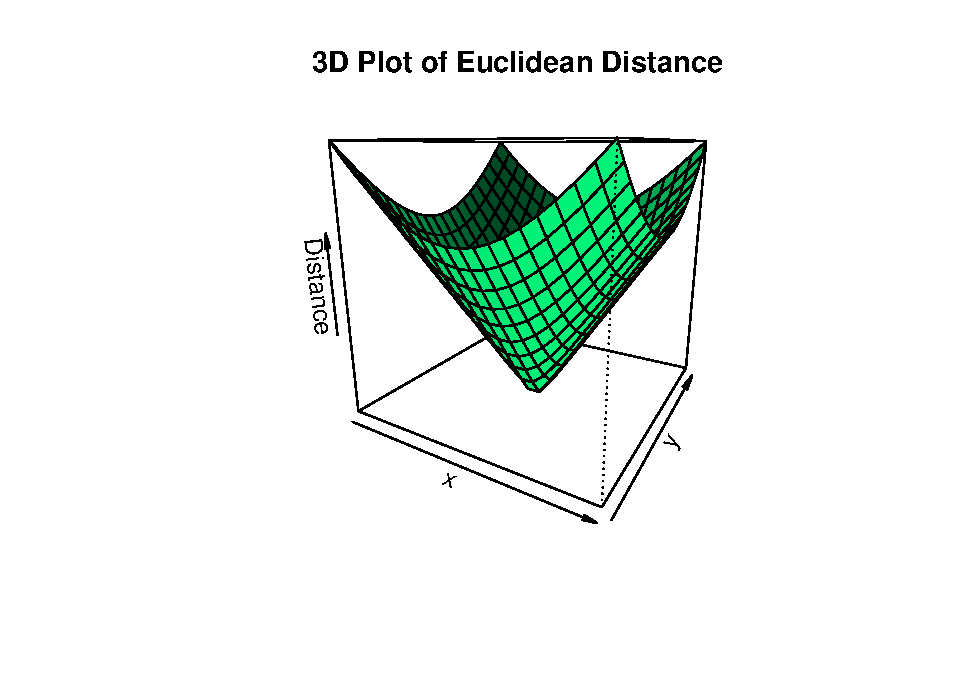
\includegraphics{week1_files/figure-latex/unnamed-chunk-2-1.pdf}

\begin{Shaded}
\begin{Highlighting}[]
\NormalTok{cone1 }\OtherTok{\textless{}{-}} \ControlFlowTok{function}\NormalTok{(x, y)\{}
\FunctionTok{sqrt}\NormalTok{(x}\SpecialCharTok{\^{}}\DecValTok{2}\SpecialCharTok{+}\NormalTok{y}\SpecialCharTok{\^{}}\DecValTok{2}\NormalTok{)}
\NormalTok{\}}

\NormalTok{x }\OtherTok{\textless{}{-}}\NormalTok{ y }\OtherTok{\textless{}{-}} \FunctionTok{seq}\NormalTok{(}\SpecialCharTok{{-}}\DecValTok{1}\NormalTok{, }\DecValTok{1}\NormalTok{, }\AttributeTok{length=} \DecValTok{20}\NormalTok{)}
\NormalTok{z }\OtherTok{\textless{}{-}} \FunctionTok{outer}\NormalTok{(x, y, cone1)}

\FunctionTok{persp}\NormalTok{(x, y, z,}
\AttributeTok{main=}\StringTok{"Perspective Plot of a Cone"}\NormalTok{,}
\AttributeTok{zlab =} \StringTok{"Height"}\NormalTok{,}
\AttributeTok{theta =} \DecValTok{30}\NormalTok{, }\AttributeTok{phi =} \DecValTok{15}\NormalTok{,}
\AttributeTok{col =} \StringTok{"springgreen"}\NormalTok{, }\AttributeTok{shade =} \FloatTok{0.5}\NormalTok{)}
\end{Highlighting}
\end{Shaded}

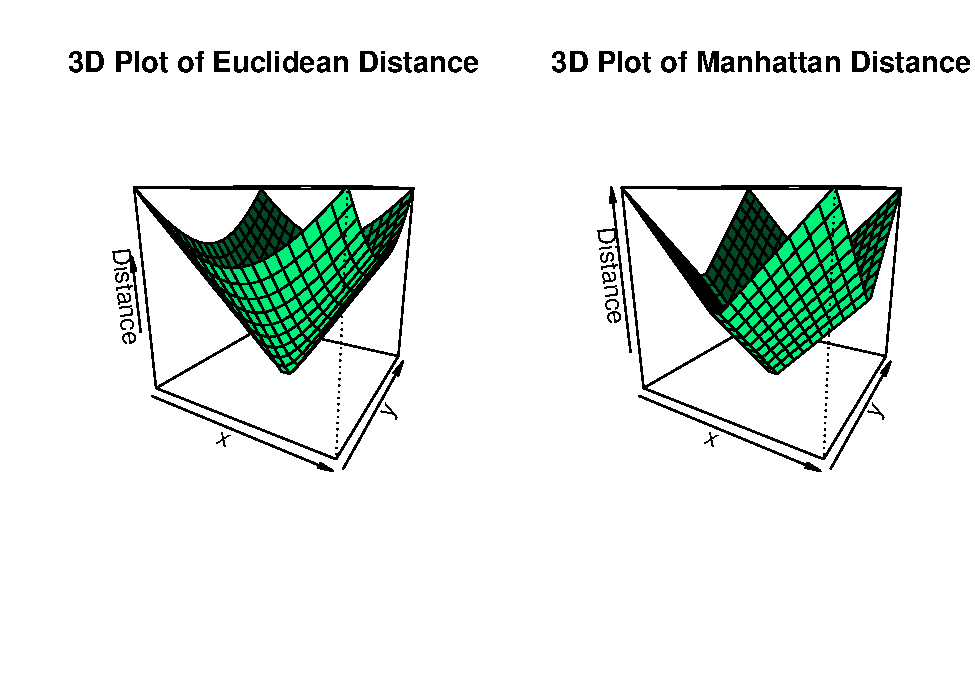
\includegraphics{week1_files/figure-latex/unnamed-chunk-3-1.pdf}

\begin{Shaded}
\begin{Highlighting}[]
\NormalTok{euclidean\_dist }\OtherTok{\textless{}{-}} \ControlFlowTok{function}\NormalTok{(point1, point2) \{}
\NormalTok{  squared\_diff }\OtherTok{\textless{}{-}}\NormalTok{ (point1 }\SpecialCharTok{{-}}\NormalTok{ point2)}\SpecialCharTok{\^{}}\DecValTok{2}
  \FunctionTok{sqrt}\NormalTok{(}\FunctionTok{sum}\NormalTok{(squared\_diff))}
\NormalTok{\}}

\NormalTok{manhattan\_distance }\OtherTok{\textless{}{-}} \ControlFlowTok{function}\NormalTok{(point1, point2) \{}
  \ControlFlowTok{if}\NormalTok{ (}\FunctionTok{length}\NormalTok{(point1) }\SpecialCharTok{!=} \FunctionTok{length}\NormalTok{(point2)) \{}
    \FunctionTok{stop}\NormalTok{(}\StringTok{"Both points should have the same number of dimensions."}\NormalTok{)}
\NormalTok{  \}}

\NormalTok{  abs\_diff }\OtherTok{\textless{}{-}} \FunctionTok{abs}\NormalTok{(point1 }\SpecialCharTok{{-}}\NormalTok{ point2)}
\NormalTok{  distance }\OtherTok{\textless{}{-}} \FunctionTok{sum}\NormalTok{(abs\_diff)}
  \FunctionTok{return}\NormalTok{(distance)}
\NormalTok{\}}

\NormalTok{x }\OtherTok{\textless{}{-}}\NormalTok{ y }\OtherTok{\textless{}{-}} \FunctionTok{seq}\NormalTok{(}\SpecialCharTok{{-}}\DecValTok{1}\NormalTok{, }\DecValTok{1}\NormalTok{, }\AttributeTok{length =} \DecValTok{20}\NormalTok{)}
\NormalTok{grid }\OtherTok{\textless{}{-}} \FunctionTok{expand.grid}\NormalTok{(}\AttributeTok{x =}\NormalTok{ x, }\AttributeTok{y =}\NormalTok{ y)  }\CommentTok{\# Create a grid of points}
\NormalTok{z\_euclidean }\OtherTok{\textless{}{-}} \FunctionTok{matrix}\NormalTok{(}\DecValTok{0}\NormalTok{, }\AttributeTok{nrow =} \FunctionTok{length}\NormalTok{(x), }\AttributeTok{ncol =} \FunctionTok{length}\NormalTok{(y))  }\CommentTok{\# Initialize the z matrix for Euclidean distance}
\NormalTok{z\_manhattan }\OtherTok{\textless{}{-}} \FunctionTok{matrix}\NormalTok{(}\DecValTok{0}\NormalTok{, }\AttributeTok{nrow =} \FunctionTok{length}\NormalTok{(x), }\AttributeTok{ncol =} \FunctionTok{length}\NormalTok{(y))   }\CommentTok{\# Initialize the z matrix for Manhattan distance}

\ControlFlowTok{for}\NormalTok{ (i }\ControlFlowTok{in} \DecValTok{1}\SpecialCharTok{:}\FunctionTok{length}\NormalTok{(x)) \{}
  \ControlFlowTok{for}\NormalTok{ (j }\ControlFlowTok{in} \DecValTok{1}\SpecialCharTok{:}\FunctionTok{length}\NormalTok{(y)) \{}
\NormalTok{    z\_euclidean[i, j] }\OtherTok{\textless{}{-}} \FunctionTok{euclidean\_dist}\NormalTok{(}\FunctionTok{c}\NormalTok{(x[i], y[j]), }\FunctionTok{c}\NormalTok{(}\DecValTok{0}\NormalTok{, }\DecValTok{0}\NormalTok{))}
\NormalTok{    z\_manhattan[i, j] }\OtherTok{\textless{}{-}} \FunctionTok{manhattan\_distance}\NormalTok{(}\FunctionTok{c}\NormalTok{(x[i], y[j]), }\FunctionTok{c}\NormalTok{(}\DecValTok{0}\NormalTok{, }\DecValTok{0}\NormalTok{))}
\NormalTok{  \}}
\NormalTok{\}}

\CommentTok{\# Create a layout of subplots to show both Euclidean and Manhattan distances}
\FunctionTok{par}\NormalTok{(}\AttributeTok{mfrow =} \FunctionTok{c}\NormalTok{(}\DecValTok{1}\NormalTok{, }\DecValTok{2}\NormalTok{))}

\CommentTok{\# Plot for Euclidean distance}
\FunctionTok{persp}\NormalTok{(x, y, z\_euclidean,}
      \AttributeTok{main =} \StringTok{"3D Plot of Euclidean Distance"}\NormalTok{,}
      \AttributeTok{zlab =} \StringTok{"Distance"}\NormalTok{,}
      \AttributeTok{theta =} \DecValTok{30}\NormalTok{, }\AttributeTok{phi =} \DecValTok{15}\NormalTok{,}
      \AttributeTok{col =} \StringTok{"springgreen"}\NormalTok{, }\AttributeTok{shade =} \FloatTok{0.5}\NormalTok{)}

\CommentTok{\# Plot for Manhattan distance}
\FunctionTok{persp}\NormalTok{(x, y, z\_manhattan,}
      \AttributeTok{main =} \StringTok{"3D Plot of Manhattan Distance"}\NormalTok{,}
      \AttributeTok{zlab =} \StringTok{"Distance"}\NormalTok{,}
      \AttributeTok{theta =} \DecValTok{30}\NormalTok{, }\AttributeTok{phi =} \DecValTok{15}\NormalTok{,}
      \AttributeTok{col =} \StringTok{"springgreen"}\NormalTok{, }\AttributeTok{shade =} \FloatTok{0.5}\NormalTok{)}
\end{Highlighting}
\end{Shaded}

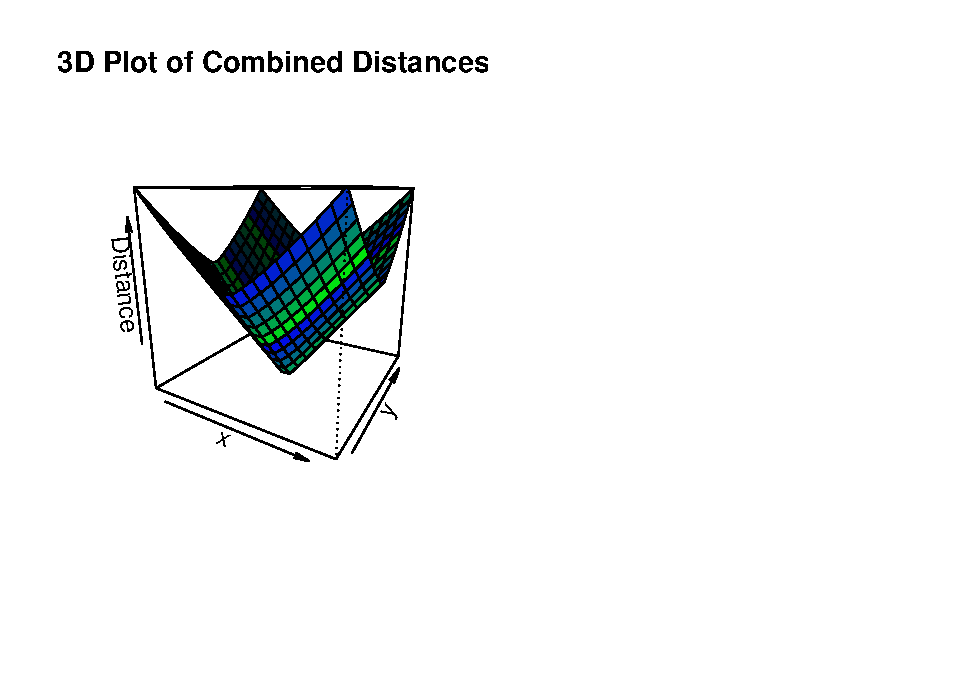
\includegraphics{week1_files/figure-latex/unnamed-chunk-4-1.pdf}

\begin{Shaded}
\begin{Highlighting}[]
\CommentTok{\# Reset the layout}
\FunctionTok{par}\NormalTok{(}\AttributeTok{mfrow =} \FunctionTok{c}\NormalTok{(}\DecValTok{1}\NormalTok{, }\DecValTok{1}\NormalTok{))}
\end{Highlighting}
\end{Shaded}

\begin{Shaded}
\begin{Highlighting}[]
\NormalTok{euclidean\_dist }\OtherTok{\textless{}{-}} \ControlFlowTok{function}\NormalTok{(point1, point2) \{}
\NormalTok{  squared\_diff }\OtherTok{\textless{}{-}}\NormalTok{ (point1 }\SpecialCharTok{{-}}\NormalTok{ point2)}\SpecialCharTok{\^{}}\DecValTok{2}
  \FunctionTok{sqrt}\NormalTok{(}\FunctionTok{sum}\NormalTok{(squared\_diff))}
\NormalTok{\}}

\NormalTok{manhattan\_distance }\OtherTok{\textless{}{-}} \ControlFlowTok{function}\NormalTok{(point1, point2) \{}
  \ControlFlowTok{if}\NormalTok{ (}\FunctionTok{length}\NormalTok{(point1) }\SpecialCharTok{!=} \FunctionTok{length}\NormalTok{(point2)) \{}
    \FunctionTok{stop}\NormalTok{(}\StringTok{"Both points should have the same number of dimensions."}\NormalTok{)}
\NormalTok{  \}}

\NormalTok{  abs\_diff }\OtherTok{\textless{}{-}} \FunctionTok{abs}\NormalTok{(point1 }\SpecialCharTok{{-}}\NormalTok{ point2)}
\NormalTok{  distance }\OtherTok{\textless{}{-}} \FunctionTok{sum}\NormalTok{(abs\_diff)}
  \FunctionTok{return}\NormalTok{(distance)}
\NormalTok{\}}

\NormalTok{x }\OtherTok{\textless{}{-}}\NormalTok{ y }\OtherTok{\textless{}{-}} \FunctionTok{seq}\NormalTok{(}\SpecialCharTok{{-}}\DecValTok{5}\NormalTok{, }\DecValTok{5}\NormalTok{, }\AttributeTok{length =} \DecValTok{20}\NormalTok{)}
\NormalTok{grid }\OtherTok{\textless{}{-}} \FunctionTok{expand.grid}\NormalTok{(}\AttributeTok{x =}\NormalTok{ x, }\AttributeTok{y =}\NormalTok{ y)  }\CommentTok{\# Create a grid of points}

\NormalTok{z\_euclidean }\OtherTok{\textless{}{-}} \FunctionTok{matrix}\NormalTok{(}\DecValTok{0}\NormalTok{, }\AttributeTok{nrow =} \FunctionTok{length}\NormalTok{(x), }\AttributeTok{ncol =} \FunctionTok{length}\NormalTok{(y))  }\CommentTok{\# Initialize the z matrix for Euclidean distance}
\NormalTok{z\_manhattan }\OtherTok{\textless{}{-}} \FunctionTok{matrix}\NormalTok{(}\DecValTok{0}\NormalTok{, }\AttributeTok{nrow =} \FunctionTok{length}\NormalTok{(x), }\AttributeTok{ncol =} \FunctionTok{length}\NormalTok{(y))   }\CommentTok{\# Initialize the z matrix for Manhattan distance}

\ControlFlowTok{for}\NormalTok{ (i }\ControlFlowTok{in} \DecValTok{1}\SpecialCharTok{:}\FunctionTok{length}\NormalTok{(x)) \{}
  \ControlFlowTok{for}\NormalTok{ (j }\ControlFlowTok{in} \DecValTok{1}\SpecialCharTok{:}\FunctionTok{length}\NormalTok{(y)) \{}
\NormalTok{    z\_euclidean[i, j] }\OtherTok{\textless{}{-}} \FunctionTok{euclidean\_dist}\NormalTok{(}\FunctionTok{c}\NormalTok{(x[i], y[j]), }\FunctionTok{c}\NormalTok{(}\DecValTok{0}\NormalTok{, }\DecValTok{0}\NormalTok{))}
\NormalTok{    z\_manhattan[i, j] }\OtherTok{\textless{}{-}} \FunctionTok{manhattan\_distance}\NormalTok{(}\FunctionTok{c}\NormalTok{(x[i], y[j]), }\FunctionTok{c}\NormalTok{(}\DecValTok{0}\NormalTok{, }\DecValTok{0}\NormalTok{))}
\NormalTok{  \}}
\NormalTok{\}}

\CommentTok{\# Combine the distances and choose different colors for each}
\NormalTok{combined\_distances }\OtherTok{\textless{}{-}}\NormalTok{ z\_euclidean }\SpecialCharTok{+}\NormalTok{ z\_manhattan}
\NormalTok{color\_palette }\OtherTok{\textless{}{-}} \FunctionTok{colorRampPalette}\NormalTok{(}\FunctionTok{c}\NormalTok{(}\StringTok{"blue"}\NormalTok{, }\StringTok{"green"}\NormalTok{))(}\DecValTok{100}\NormalTok{)  }\CommentTok{\# Choose colors for mapping distances}

\CommentTok{\# Create a layout of subplots}
\FunctionTok{layout}\NormalTok{(}\FunctionTok{matrix}\NormalTok{(}\FunctionTok{c}\NormalTok{(}\DecValTok{1}\NormalTok{, }\DecValTok{2}\NormalTok{), }\AttributeTok{nrow =} \DecValTok{1}\NormalTok{))}

\CommentTok{\# Plot both distances on the same 3D plane with different colors}
\FunctionTok{persp}\NormalTok{(x, y, combined\_distances,}
      \AttributeTok{main =} \StringTok{"3D Plot of Combined Distances"}\NormalTok{,}
      \AttributeTok{zlab =} \StringTok{"Distance"}\NormalTok{,}
      \AttributeTok{theta =} \DecValTok{30}\NormalTok{, }\AttributeTok{phi =} \DecValTok{15}\NormalTok{,}
      \AttributeTok{col =}\NormalTok{ color\_palette, }\AttributeTok{shade =} \FloatTok{0.5}\NormalTok{)}

\CommentTok{\# Reset the layout}
\FunctionTok{layout}\NormalTok{(}\DecValTok{1}\NormalTok{)}
\end{Highlighting}
\end{Shaded}

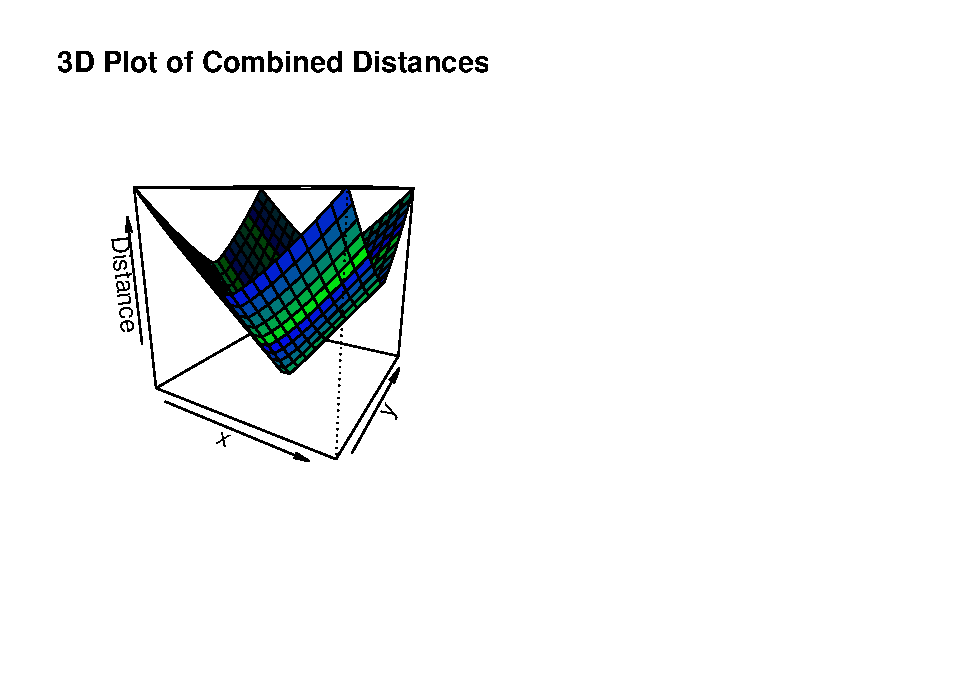
\includegraphics{week1_files/figure-latex/unnamed-chunk-5-1.pdf}

\begin{Shaded}
\begin{Highlighting}[]
\CommentTok{\# Include the script from the R directory}
\NormalTok{project\_path }\OtherTok{\textless{}{-}} \FunctionTok{here}\NormalTok{()}
\FunctionTok{source}\NormalTok{(}\FunctionTok{here}\NormalTok{(}\StringTok{"R"}\NormalTok{, }\StringTok{"utils.R"}\NormalTok{))}
\end{Highlighting}
\end{Shaded}

\begin{Shaded}
\begin{Highlighting}[]
\NormalTok{?entropy}
\end{Highlighting}
\end{Shaded}

\begin{verbatim}
## No documentation for 'entropy' in specified packages and libraries:
## you could try '??entropy'
\end{verbatim}

\end{document}
